
%!TEX ROOT=main.tex


\part{Software}
\label{chap:software}
\section{Introduction}
The control program for both the transmitter and the car is written in C language. It utilizes the STM32 HAL (Hardware Abstraction Layer) libraries, and the STM32CubeMX graphical utility was used to set up the necessary initialization and project files and generate code for peripheral configuration.

STM32 HAL driver library provides a set of APIs to simplify interaction with all the peripherals and thus the user application implementation. The HAL driver layer implements run-time failure detection to increase robustness. HAL APIs are available for all peripherals. Also, the API ensures high portability across different STM32 families \cite{hal}.

STM32CubeMX is a graphical tool that provides a convenient user interface to configure the microcontroller. It allows a simple configuration of pin assignments, peripherals, or the clock tree, and the corresponding C initialization code generation. It also packs middleware stacks, such as USB, FatFs, or TCP/IP. This tool notably speeds up the process of microcontroller configuration and allows the user to focus on the application \cite{cubemx}.

The control program is almost exclusively interrupt-driven. Emphasis has been placed on program execution speed to ensure a high frequency of control commands and, therefore, smooth car control.

\section{File structure}
\todo

\section{Transmitter}
\subsection{Peripherals and pin configuration}
\label{sub:tx_conf}
\begin{figure}[t]
\centering
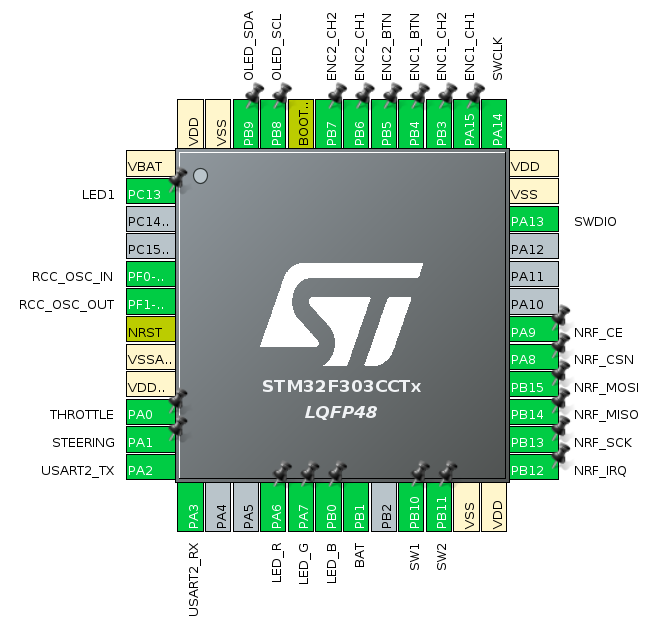
\includegraphics[width=0.7\linewidth]{fig/tx_pin_assignments.png}
\caption{Transmitter pin assignments}
\label{fig:tx_conf}
\end{figure}
The microcontroller runs at \SI{72}{\MHz} with a clock source set to a \SI{12}{\MHz} external crystal oscillator.

ADC1 channels 1 and 2 are used to measure the output voltage from control potentiometers. ADC operates with 12-bit resolution in continuous conversion mode with DMA enabled in circular mode with continuous requests to manipulate the data. Once the ADC conversion is started, it remains active, and DMA repeatedly fills the buffer with measured data. Sampling time is the highest possible 601.5 cycles, and software averaging is used to acquire stable measurements.

ADC3 uses channel 1 to measure the LiPo battery voltage and channel Vrefint to measure the internal reference voltage. Again, the resolution is 12-bit, continuous conversion mode is enabled, and DMA is utilized to transfer data from peripheral to memory. In this mode, the ADC remains active until DMA fills the whole data buffer. The sampling time for channel 1 is $601.5$ cycles, and for channel Vrefint $181.5$ cycles.

The communication module is connected to the SPI2 bus operating in full-duplex master mode. Baud rate is set to \SI{9}{\mega\bit\per\second}, and the data size is standard 8 bits. 'NRF\_IRQ' pin is configured in external interrupt mode with rising edge detection. The rest of the 'NRF' pins are simple outputs.

Quadrature rotary encoders utilize timers TIM2 and TIM4, which are in Encoder mode. This mode is designed specially to interface quadrature encoders with out-of-phase output signals. Encoder push-button pins are configured in external interrupt mode with rising edge detection.

SW1 and SW2 pins belong to the DIP switch and are configured in external interrupt mode with both rising and falling edge detection.

USART2 peripheral is configured as debug serial port. Baud rate is set to \SI{921600}{\bit\per\second} with 8 bits word length and one stop bit.

I2C1 in Fast Mode Plus with a frequency of \SI{1}{\MHz} connects the OLED display, and LED pins are simple outputs. Furthermore, TIM6 at \SI{1}{\Hz} and TIM16 at \SI{4}{\Hz}, both timers with interrupts enabled, are used for basic timing purposes.

Figure \ref{fig:tx_conf} shows the complete pinout in STM32CubeMX.

\subsection{Application start}
The program starts with auto-generated initialization of all necessary peripherals. Debug UART is enabled after start by default. Afterward, an orange LED visible from the backside of the transmitter is turned on to indicate application initialization.

First, the OLED display is initialized, and the project logo is displayed. At the same time, a greeting is sent via UART, and the RGB LED flashes through each channel. Automatic self-calibration of both ADCs follows, and the Vrefint calibration value is obtained from the appropriate register. This value is later used to calculate VDDA. Then the communication module is initialized with parameters defined in \textit{platform.h}.

After that, the ADC responsible for reading values of control potentiometers is started in circular DMA mode, as described in section \ref{sub:tx_conf}. Processing of the data is explained in section \ref{sub:adc}.

In the final part of initialization, all the timers, including the timers used for quadrature encoders, are started in interrupt mode. Then the UART is deinitialized depending on the Switch1 state, the orange LED is turned off to indicate that initialization is done, and the program enters the main control loop.

\subsection{Main control loop}
The control loop is designed to be as non-blocking and interrupt-driven as possible. Therefore, it consists of a set of 'if' blocks. However, some parts remained blocking. The reason is some of the drivers are blocking and do not allow the use of DMA. Rewriting them was hardly possible or too time-consuming. This is especially true for OLED refreshing, which takes the longest time. Execution of given 'if' block is controlled by flags, internally boolean values, set by appropriate interrupt routines.

The \textit{'trigger\_data\_rdy'} flag is set by ADC interrupt routines, and it controls the execution of the first block. It processes and averages measured data from control potentiometers and recalculates the values using hardware limits for direct usage in the car.

The block controlled by the \textit{'adc\_data\_bat\_rdy'} flag is similar to the previous block. First, it averages the measured Vrefint and battery voltage data. The next step is VDDA calculation:
\begin{equation}
	V_{DDA} = \frac{\SI{3.3}{\V} \cdot Vrefint_{cal}}{Vrefint_{meas}}\ ,
\end{equation}
where $Vrefint_{cal}$ is a factory-trimmed value obtained from register and $Vrefint_{meas}$ is measured internal reference voltage. The formula was taken from Section 15.3.32 in \cite{f303_ref}. This computed value is used to convert the ADC battery measurement to the actual voltage. The corresponding ADC sets the flag.

\subsection{ADC data processing}
\label{sub:adc}
A feature similar to 'double buffering' is implemented to process data from ADC in circular mode. It is not implemented as two separate buffers but as a single 1024 bytes long buffer. It utilizes the ADC ability to send notifications when the buffer is half-full and when it is full.

ADC is enabled and DMA starts filling the buffer with data. Once the buffer is half-full, the appropriate interrupt is triggered, and MCU is signaled to start processing the first half of the buffer. The DMA still fills the buffer with new data.

When the DMA fills the buffer completely, the appropriate interrupt is triggered, and the DMA starts filling the buffer from the beginning with new measurements. This state is again signaled to the MCU, which starts processing the second half of the buffer while the DMA fills the first half.

Whether the first or the second half is to be processed is controlled by an integer offset that is set in the interrupt routine. Hence, this method is fast as the DMA still fills the same buffer and does not need to be reconfigured, which would add additional overhead.

This approach is repeated, ensuring that the new measurements do not overwrite the values already in the buffer and, therefore, do not affect the value obtained.

\subsection{UART debug prints}
\todo




\section{Car}
\subsection{Peripherals and pin configuration}
\begin{figure}[t]
\centering
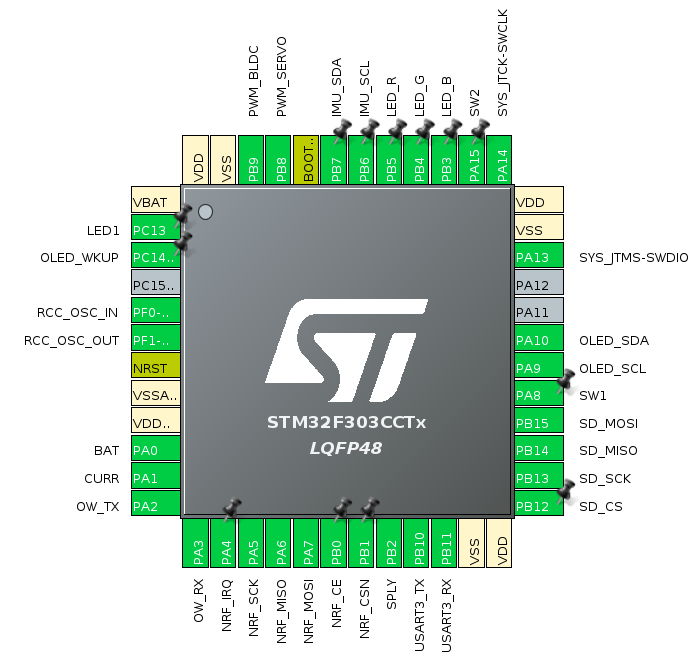
\includegraphics[width=0.75\linewidth]{fig/car_pin_assignments.png}
\caption{Car pin assignments}
\label{fig:car_conf}
\end{figure}
Some of the settings are similar to transmitter settings since both microcontrollers are the same STM32F303CCT6. The microcontroller runs at \SI{72}{\MHz} with a clock source set to an \SI{8}{\MHz} external crystal oscillator.

Channels 2 and 3 of timer TIM8 are used to generate PWM and therefore control the car. Prescaler and counter period values are calculated to represent the pulse width in microseconds. That means the counter value of e.g. $1500$ equals \SI{1500}{\micro\second} pulse width, which is convenient for control application implementation.

ADC1 channels 1 and 2 are used to measure the LiPo battery voltage and output voltage from the current sensor. ADC operates with 12-bit resolution in continuous conversion mode with DMA enabled. Sampling time is again the highest possible $601.5$ cycles to acquire stable measurements.

ADC2 measures the Vrefint channel to obtain the internal reference voltage and channel 12 to obtain the BEC output voltage. The resolution is also 12-bit, and continuous conversion mode with DMA is enabled. The sampling time for channel Vrefint is $181.5$ cycles and $601.5$ cycles for channel 12.

The communication module is connected to the SPI1 bus operating in full-duplex master mode. Baud rate is set to \SI{9}{\mega\bit\per\second}, and the data size is standard 8 bits. 'NRF\_IRQ' pin is configured in external interrupt mode with rising edge detection. The rest of the 'NRF' pins are simple outputs.

As STM32F303 does not support the SDIO interface, the SD card is connected via the SPI2 peripheral. The baud rate is only \SI{281.25}{\kilo\bit\per\second} after reset, but once the SD card is initialized, it is increased to \SI{9}{\mega\bit\per\second}.

I2C2 in Fast Mode Plus with a frequency of \SI{1}{\MHz} connects the OLED display. IMU unit is served by I2C1 in Fast Mode with a frequency of \SI{400}{\kHz}.

1-Wire bus necessary to communicate with the DS18B20 temperature sensor is implemented using USART2 peripheral and DMA. The implementation is described in section *sec*. [\todo section]

SW1 and SW2 pins belong to the DIP switch and are configured in external interrupt mode with both rising and falling edge detection.

USART3 peripheral is configured as debug serial port. Baud rate is set to \SI{921600}{\bit\per\second} with 8~bits word length and one stop bit.

LED pins are simple outputs. Pins PA11 and PA12 are not used in the project's current state but are reserved for a USB peripheral for possible future expansion with a control computer.

Figure \ref{fig:car_conf} shows the complete pinout in STM32CubeMX.